\documentclass{article}
\usepackage{fullpage,amsmath,amsthm,graphicx,enumitem,amsfonts}
\usepackage{multicol}
\usepackage{booktabs}
\usepackage{tikz}
\usepackage{xcolor}
\newcommand{\tb}[1]{\textcolor{cyan}{[TB: #1]}}
\newcommand{\solutionspace}[1]{
    \newpage
    (Solution space for question #1)
    \newpage
    (Solution space for question #1)
    \clearpage
}
\DeclareMathOperator*{\argmax}{arg\!\max}
\DeclareMathOperator*{\argmin}{arg\!\min}

\newcommand{\zs}[1]{{\color{blue}[ZS: #1]}}

\usepackage[normalem]{ulem} % only for \sout in \zsedit below
\newcommand{\zsedit}[2]{{\color{blue} \sout{#1}#2}}

\theoremstyle{definition}
\newtheorem{thm}{Theorem}
\newtheorem{question}[thm]{Question}
\newenvironment{solution}{\noindent\textit{Solution:}}{}

\title{ASEN 5264 Decision Making under Uncertainty\\
       Exam 1 (2026): Probabilistic Models and MDPs}


\begin{document}
\maketitle


\begin{question} (10 pts)
Consider the following Bayesian network made up of binary random variables:
\begin{center}
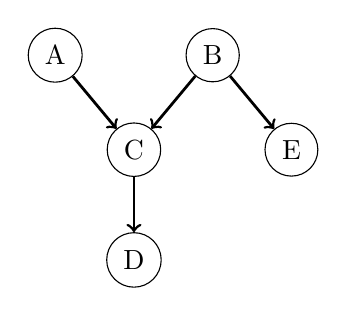
\begin{tikzpicture}
    \node[shape=circle,draw=black] (A) at (0,0) {A};
    \node[shape=circle,draw=black] (B) at (2,0) {B};
    \node[shape=circle,draw=black] (C) at (1,-1.2) {C};
    \node[shape=circle,draw=black] (D) at (1,-2.6) {D};
    \node[shape=circle,draw=black] (E) at (3,-1.2) {E};

    \path [->,line width=1pt] (A) edge (C);
    \path [->,line width=1pt] (B) edge (C);
    \path [->,line width=1pt] (C) edge (D);
    \path [->,line width=1pt] (B) edge (E);
\end{tikzpicture}
\end{center}


\begin{enumerate}[label=\alph*)]
    \item Is it possible to conclude from the structure alone that $C \perp E \mid B$?
    \item Is it possible to conclude from the structure alone that $A \perp E \mid C$?

    \item Suppose that you are given the probability distributions $P(A)$, $P(B)$, $P(C \mid A, B)$, and $P(D \mid C)$. Write down a symbolic expression for the value of $P(A=1 \mid D=1)$ in terms of the values in the given distributions (e.g. $P(D=1 \mid C=1)$).
\end{enumerate}
\end{question}



\clearpage

\begin{question}(25 pts)
    An Olympic snowboarder is traveling down an infinitely long half-pipe seeking to maximize her expected score with a discount rate of $\gamma=0.9$. She has two tricks in her repertoire, an easy one and a difficult one. When she attempts a trick, she may either fall and get a score of zero or land and get the score in the table below. The easy trick always has a 80\% successful landing rate.
    After a successful landing of either trick, the snowboarder is stoked, and the difficult trick has an 80\% successful landing rate, but has only a 70\% successful landing rate otherwise.

    \begin{center}
    \begin{tabular}{lc}
        \toprule
        Trick & Score \\
        \midrule
        Easy & 70 \\
        Difficult & 90 \\
        \bottomrule
    \end{tabular}
    \end{center}
\end{question}

\begin{enumerate}[label=\alph*)]
    \item Formulate this problem as a Markov decision process by writing down:
    \begin{itemize}[noitemsep]
        \item the state space,
        \item the action space,
        \item the transition probabilities,
        \item the reward function (you can define $R(s,a,s')$ or $R(s, a)$, the expected immediate reward for the action).
    \end{itemize}

    \item If the snowboarder has just fallen, which action is the greedy action, i.e. which action has the highest \emph{immediate} reward, $R(s, a)$? Is there any reason why the Olympian wouldn't want to take this greedy action? Explain in one or two sentences.

    \item Let $\tilde{\pi}$ be a policy that attempts the easy trick after a fall and the difficult trick after a landing. Use the symbols you defined above to write down this policy as a function.

    \item Show how you would determine whether $\tilde{\pi}$ is better than a policy that always takes the greedy action. Substitute numbers into equations wherever possible, but you do not need to solve the equations.

    \item Suppose the snowboarder's coach suggests that she should follow a stochastic policy $\tilde{\pi}'$ which is the same as $\tilde{\pi}$ except that, after a fall, she attempts a difficult trick 10\% of the time. Is it possible that $\tilde{\pi}'$ is the unique optimal policy?
\end{enumerate}

\clearpage


\begin{question}\label{q:td-control} (15 pts)
Consider learning a state-action value function $Q(s,a)$.
Let $\gamma=0.9$ and learning rate $\alpha=0.5$. States are $\mathcal{S} = \{1,2,3\}$, and actions are $\mathcal{A}=\{a,b\}$.

You are given the current Q-table:
\[
\begin{array}{c|cc}
 & a & b\\ \hline
1 & 1.0 & 0.0\\
2 & 4.0 & 6.0
\end{array}
\qquad
\text{and } Q(3,a)=Q(3,b)=0 \text{ for terminal state } 3.
\]

An exploration policy generates the following trajectories:
\begin{align}
    \tau^{(1)} &= (s_1=1,\ a_1=a,\ r_1=0,\ s_2=2,\ a_2=a,\ r_2=5,\ s_3=3)\\
    \tau^{(2)} &= (s_1=1,\ a_1=a,\ r_1=-4,\ s_2=3)\\
    \tau^{(3)} &= (s_1=1,\ a_1=b,\ r_1=1,\ s_2=2,\ a_2=b,\ r_2=-8,\ s_3=3)
\end{align}

\begin{enumerate}[label=\alph*)]
    \item Using one update at each transition in the trajectory $\tau^{(1)}$, calculate the new state-action values $Q(1,a)$ and $Q(2,a)$ with:
    \begin{enumerate}[label=\roman*)]
        \item Q-learning,
        \item SARSA.
    \end{enumerate}
    \item If we are executing maximum likelihood model based tabular reinforcement learning and have observed the three trajectories above, what MDP do we solve to improve the policy? (Define the transition and reward models for this MDP.)
\end{enumerate}


\end{question}
\vspace{3cm}
\begin{question} (10 pts)
    Let $B$ denote the Bellman operator for a finite discrete MDP, defined by
        $B[U](s) = \max_{a\in A} [R(s, a) + \gamma \sum_{s'} T(s' \mid s,a) \, U(s')]$.
    Suppose that we are solving an MDP with discount $\gamma=0.9$ and rewards bounded as $-5 \le R(s,a) \le 10\; \forall s,a$. After $k$ iterations of value iteration, we have a Bellman residual of 0.2, i.e.,
    \[
        \|B[U_k] - U_k\|_\infty = 0.2.
    \]
    \begin{enumerate}[label=\alph*)]
        \item A student claims that there exists a state $s$ such that the optimal value satisfies $U^*(s)=200$. Is it possible to prove or disprove the claim with the given information? Justify your answer.
        \item Given the information above, is it possible that the max-norm distance between $U_k$ and the optimal value function $U^*$ is 3, that is, $\|U_k - U^*\|_\infty = 3$? Justify your answer. (Hint: derive an upper bound for $\|U_k - U^*\|_\infty$ given the Bellman residual.)
    \end{enumerate}
\end{question}


\end{document}
